% Farben aus dem Bild definieren
\definecolor{coverblue}{RGB}{0,115,165}
\definecolor{covergray}{RGB}{58,58,60}
\thispagestyle{empty}

\begin{tikzpicture}[remember picture,overlay]
  % Vertikaler Text auf dem grauen Balken
    \node[rotate=90, anchor=south,
        font=\sffamily\bfseries\fontsize{54}{64}\selectfont,
        text=coverblue] % oder text=coverblue, wenn du das Blau als Schrift willst
    at ($(current page.west) + (3cm,0cm)$)
        {MATHEMATIK -- MATURA};

    \node[text=black, anchor=west, align=right]
    at ($(current page.north) - (4.5cm,7cm)$)
        { 
            \begin{tabular}{r}
                \Huge Skriptum zur AHS-Matura \\[0.5cm]
                \Large \today \\[0.5cm]
                \Large Nils Schlager
            \end{tabular}
        };


    \draw[rounded corners=10pt, coverblue,line width=6pt] 
    ($(1.5,-1)$) rectangle ($(3,-1)+(20,-6)$);    

    \node[text=black, anchor=west, align=right]
    at ($(current page.north) - (-5cm,28cm)$) {Version 1.0.0};
    

\def\xoffset{1}   % change this to shift everything in x
\def\yoffset{0}   % change this to shift everything in y

\node[opacity=0.5] at ($ (8,-16) + (\xoffset,\yoffset) $) 
  {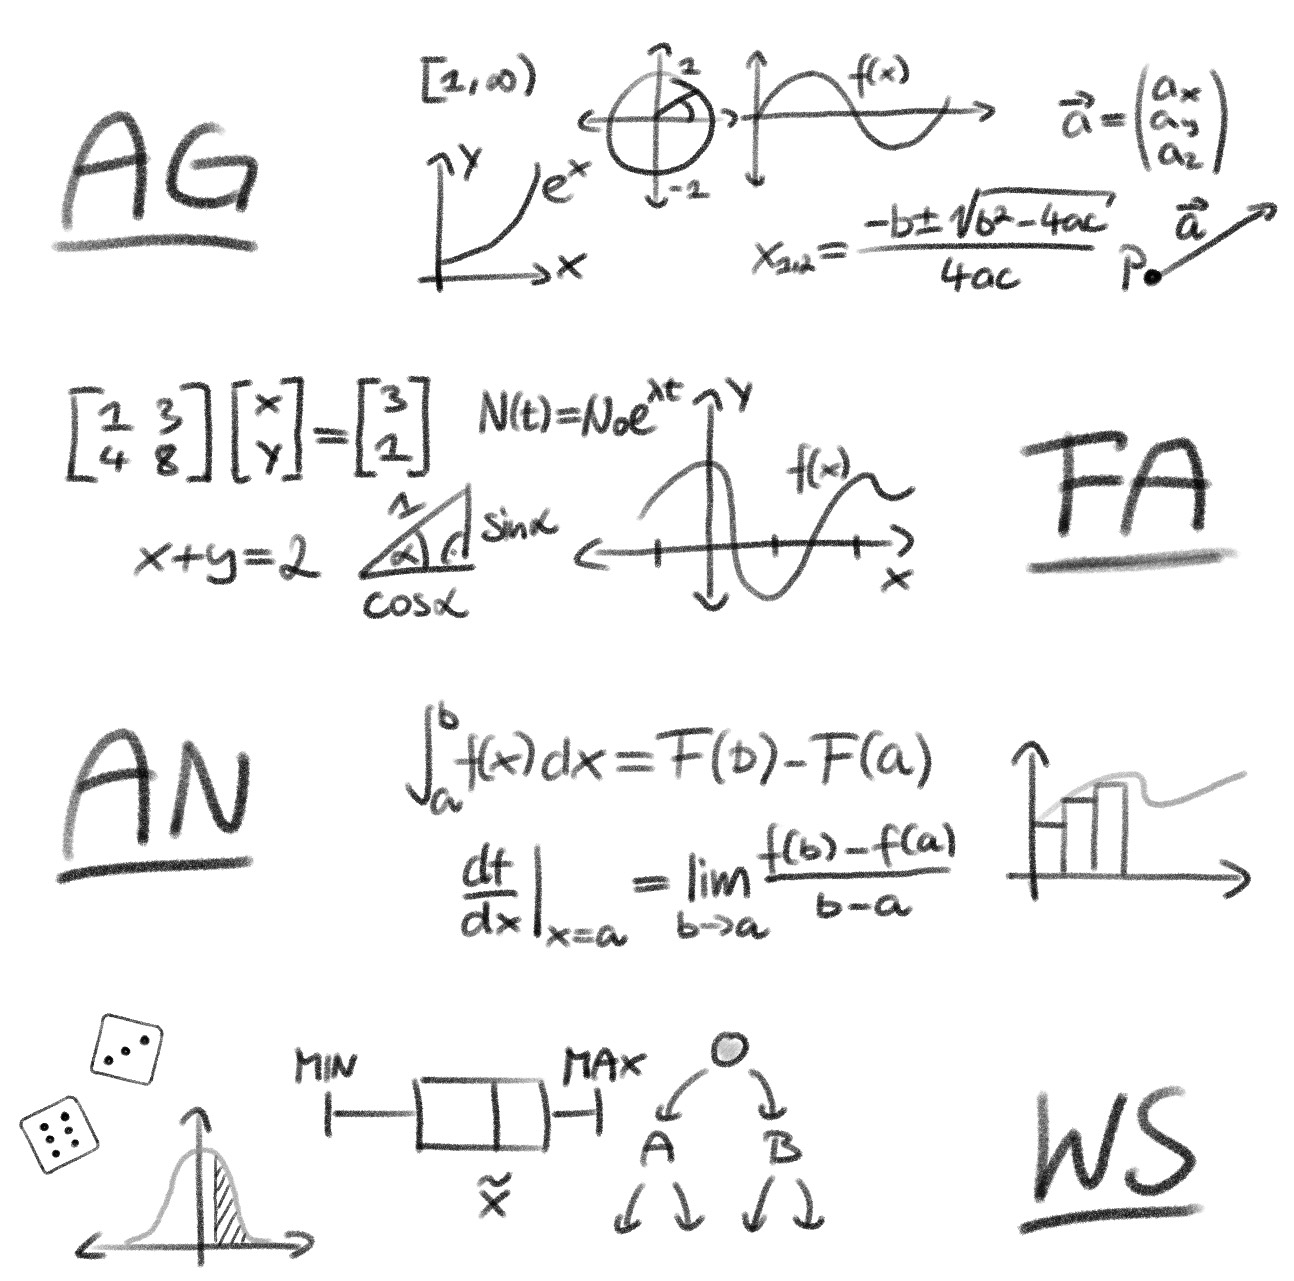
\includegraphics[width=14cm]{background.png}};

\draw[rounded corners=8pt] 
  ($ (1,-9.5) + (\xoffset,\yoffset) $) 
  rectangle 
  ($ (1,-9.5) + (3.5,-3) + (\xoffset,\yoffset) $);

\draw[rounded corners=8pt] 
  ($ (5,-9.5) + (\xoffset,\yoffset) $) 
  rectangle 
  ($ (5,-9.5) + (10,-3) + (\xoffset,\yoffset) $);

\draw[rounded corners=8pt] 
  ($ (11.5,-13) + (\xoffset,\yoffset) $) 
  rectangle 
  ($ (11.5,-13) + (3.5,-3) + (\xoffset,\yoffset) $);

\draw[rounded corners=8pt] 
  ($ (1,-13) + (\xoffset,\yoffset) $) 
  rectangle 
  ($ (1,-13) + (10,-3) + (\xoffset,\yoffset) $);

\draw[rounded corners=8pt] 
  ($ (1,-16.5) + (\xoffset,\yoffset) $) 
  rectangle 
  ($ (1,-16.5) + (3.5,-3) + (\xoffset,\yoffset) $);

\draw[rounded corners=8pt] 
  ($ (5,-16.5) + (\xoffset,\yoffset) $) 
  rectangle 
  ($ (5,-16.5) + (10,-3) + (\xoffset,\yoffset) $);

\draw[rounded corners=8pt] 
  ($ (11.5,-20) + (\xoffset,\yoffset) $) 
  rectangle 
  ($ (11.5,-20) + (3.5,-3) + (\xoffset,\yoffset) $);

\draw[rounded corners=8pt] 
  ($ (1,-20) + (\xoffset,\yoffset) $) 
  rectangle 
  ($ (1,-20) + (10,-3) + (\xoffset,\yoffset) $);
\end{tikzpicture}
\clearpage